\documentclass[a4paper, 12pt]{article}
\author{Justin L. Clough}
\title{Analysis of Flutter Importance \\ for a Typical High Speed Panel}
\usepackage[margin=1in]{geometry}
\usepackage{float}
\usepackage{subfigure}
\usepackage[justification=centering]{caption}
\usepackage{enumerate}
\usepackage{multirow}
\usepackage{listings}
\lstset{
    escapechar=`,
    language=C++,
    numbers=left,
    tabsize=2,
    prebreak=\raisebox{0ex}[0ex][0ex]{\ensuremath{\hookleftarrow}},
    frame=single,
    breaklines=true,
}
\usepackage{graphicx}
\graphicspath{ {./} }
\usepackage{nameref}
\usepackage{amsmath}
\usepackage{amssymb}
\usepackage{amsfonts}
\usepackage[linesnumbered,ruled]{algorithm2e}
\usepackage{tikz}
\usetikzlibrary{calc,patterns,decorations.pathmorphing,decorations.markings,positioning,automata}
\usepackage{pgfplots}
\usepackage{pgfplotstable}
\usepackage{makecell}
\usepackage{verbatim}

\begin{document}
\maketitle

The importance of flutter\footnote{\emph{flutter} in the scope of this paper
 is taken to mean the oscillatory motion of an object
 due to its inertia and the interactions with the 
 surrounding fluid.
 }
is analyzed for a typical high speed panel.
This analysis follows the method of non-dimensional dynamic pressure, $\lambda$, 
outlined by Mei et al. \cite{bib:nasa_paper_Mei}.
According to this paper, the behavior of a simply-supported panel with uniform temperature
interacting with high-speed flow can be found by knowing $\lambda$
and the ratio of the operating temperature with respect to a critical temperature.
The critical temperature is the temperature at which a static panel would buckle
due to its thermal stresses. 
The map between dynamic pressure, temperature ratio, and panel behavior is shown in
Figure \ref{fig:lambda_map}.

\begin{figure}[H]
  \centering
  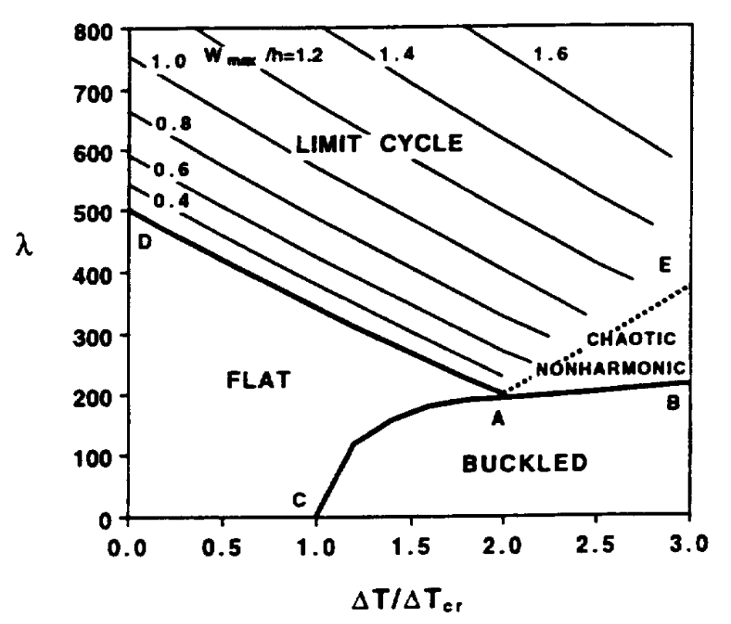
\includegraphics[width=0.8\textwidth]{nasa_lambda_T_areas}
  \caption{Plot of dimensionless dynamic pressure and temperature ratio 
           for a simply supported panel. 
           Image borrowed from Fig. 2 of \cite{bib:nasa_paper_Mei}.
           $W_{max}/h$ refers to the maximum out of plane displacement ($W_{max}$)
           as compared to panel thickness ($h$).
          }
  \label{fig:lambda_map}
\end{figure}

\noindent
The non-dimensional dynamic pressure expression is shown in Equation \ref{eq:lambda}.
This relation is originally shown as Equation 4.2 of \cite{bib:nasa_paper_Mei}.

\begin{equation}
\lambda = \frac{2 q_a a^3}{\beta D_{110}}
\label{eq:lambda}
\end{equation}

\noindent
In Equation \ref{eq:lambda}, 
$q_a$ is the traditional measure of dynamic pressure 
(as shown in Equation \ref{eq:dynamic_pressure}),
$a$ is the length of the panel in the direction of the flow,
$\beta$ is a measure of the airspeed ($\beta = \sqrt{M_{\infty}^2 -1}$),
$M_{\infty}$ is the Mach number of the flow,
and
$D_{110}$ is a measure of the panel stiffness shown in Equation \ref{eq:D_110}.
The traditional dynamic pressure equation is shown in Equation \ref{eq:dynamic_pressure}.

\begin{equation}
q_a = \frac{\rho_a V^2}{2}
\label{eq:dynamic_pressure}
\end{equation}

\noindent
The density of the air is $\rho_a$ and the air speed velocity is $V$.
The panel stiffness measure, $D_{110}$, is shown in Equation \ref{eq:D_110} 
for homogeneous and isotropic panels.

\begin{equation}
D_{110} = E Q
\label{eq:D_110}
\end{equation}

\noindent
The Young's Modulus of the material is $E$ and $Q$ is the first area moment
with respect to the area facing the flow.
Two panels are analyzed; 
the first is a representative panel of interest,
the second is one from a report by LaFontaine et al. \cite{bib:LaFontaine}.
The second panel is used to double check this analysis method's results.  

The first panel considered has geometry borrowed 
from Plews and Duarte \cite{bib:Plews}.
The original panel and Engineering Sketch Pad (ESP) approximation are 
show in Figure \ref{fig:panel_geom}.
The ESP mock-up was made to measure cross-sectional 
properties of the geometry.
Only one of the stiffened sections was modeled and 
the hat stiffener was approximated as a C-channel.

\begin{figure}[H] 
  \centering
  \subfigure[Panel from Fig. 19 of Plews and Duarte. Dimensions in inches.]{
    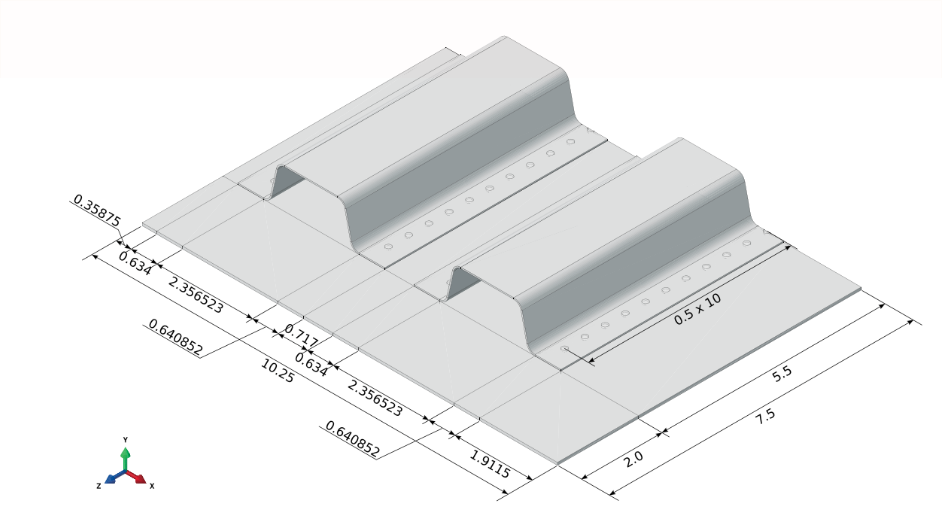
\includegraphics[width=0.45\textwidth]{plews_panel}
  }
  \subfigure[Approximation made with ESP.]{
    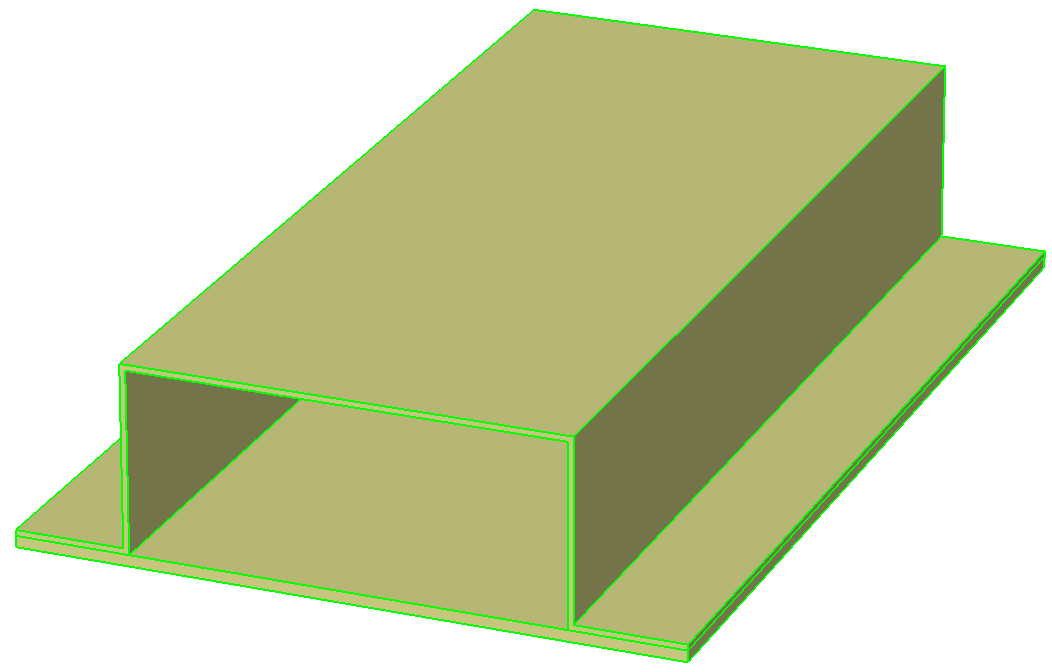
\includegraphics[width=0.45\textwidth]{esp_panel}
  }
  \caption{Original panel geometry and channel approximation.
           A larger image of (a) is shown in Appendix \ref{app:big_image}.}
  \label{fig:panel_geom}
\end{figure}

\noindent
The approximation in ESP has a length of 139.7 mm (5.5 in). 
The skin thickness was 1.59 mm and the thickness of the stiffener 
sheet was 0.81 mm for both geometries. 
The interior channel width was 59.8 mm (2.35 in) for the C-channel.
Both stiffeners had an interior hat height of 25.3 mm (1.0 in).
The outer edges of both panels include the thickness of the skin 
and stiffener sheets.
The fluid conditions used were an air density of 1.0 Kg/m$^3$ 
(corresponding to an altitude of 70,000 ft) 
and airspeed of Mach 5.0; 
these values are based on the publicly available cruising speed 
and altitude of the X-51 \cite{bib:x51_factsheet}.
The material properties of Ti6Al4V were used; 
Young's modulus was taken to be 113.8 GPa \cite{bib:ti6al4v}.

Evaluating Equation \ref{eq:lambda} with the hat-stiffened panel
parameters yields the following:

\begin{align*}
\lambda 
 &= \frac{2 q_a a^3}{\beta D_{110}} \\
 &= \frac{\rho_a V^2 a^3}{ (\sqrt{M_{\infty}^2 -1}) E Q} \\
 &= \frac{(1.0 \text{Kg}/\text{m}^3) (1701 \text{m}/\text{s})^2 (0.1397 \text{m})^3}{ \sqrt{5.0^2 -1} (113.8 \text{GPa}) (1.04\times 10^{-6} \text{m}^3)} \\
 &\approx 0.014
\end{align*}

\noindent
Referring back to Figure \ref{fig:lambda_map}, 
a dimensionless dynamic pressure of 0.014 
is either static or buckled for all operating temperatures.
A panel of this configuration is not expected to flutter.

The second panel is a plate borrowed from LaFontaine et al. \cite{bib:LaFontaine}.
The panel geometry is 1 m long with a 2.5 mm cross section.
It is made of Aluminum alloy 7075 with Young's modulus of 71.0 GPa.
The free stream velocity is Mach 5.3.
It was assumed the air had a density of 1.0 Kg/m$^3$ for both panels.
Evaluating Equation \ref{eq:lambda} with this panel
parameters yields the following:

\begin{align*}
\lambda 
 &= \frac{2 q_a a^3}{\beta D_{110}} \\
 &= \frac{\rho_a V^2 a^3}{ (\sqrt{M_{\infty}^2 -1}) E Q} \\
 &= \frac{(1.0 \text{Kg}/\text{m}^3) (1818 \text{m}/\text{s})^2 (1 \text{m})^3}{ \sqrt{5.3^2 -1} (71.0 \text{GPa}) (1.56\times 10^{-8} \text{m}^3)} \\
 &\approx 1140
\end{align*}

\noindent
Referring back to Figure \ref{fig:lambda_map}, 
a dimensionless dynamic pressure of 1140
corresponds to limit cycle oscillations for all operating temperatures;
this matches the findings of the original study.


\newpage
\begin{thebibliography}{99}
\bibitem{bib:nasa_paper_Mei}
Chuh Mei,
K. Abdel-Motagaly,
and R. Chen.
Review of Nonlinear Panel Flutter at Supersonic and Hypersonic Speeds.
CEAS/AISS/ICASE/NASA Langley International Forum on Aeroelasticity and Structural Dynamics 1999. 
June 1999.

\bibitem{bib:LaFontaine}
Jonathen H. LaFontaine,
Abhijit Gogulapati,
and Jack J. McNamara.
Effects of Strain Hardening on Response of Skin Panels in Hypersonic Flow.
AIAA Journal Vol. 54, No. 6.
June 2016.

\bibitem{bib:Plews}
J. A. Plews
and C. A. Duarte.
A two-scale generalized finite element approach for modeling localized thermoplasticity.
International Journal for Numberical Methods in Engineering.
March 2016.

\bibitem{bib:x51_factsheet}
Factsheets: X-51A Waverider.
U.S.Air Force. 
Retrieved September 6th, 2018. 
Available from: www.af.mil/About-Us/Fact-Sheets/Display/Article/104467/x-51a-waverider.

\bibitem{bib:ti6al4v}
Aerospace Specification Metals Inc.
Titanium Ti-6Al-4V (Grade 5), Annealed Material Data Sheet.
Retrieved September 6th, 2018.
Available from: asm.matweb.com/search/SpecificMaterial.asp?bassnum=mtp641

\end{thebibliography}

\newpage
\appendix
\section{Panel from Plews and Duarte.}\label{app:big_image}

\begin{figure}[H]
  \centering
  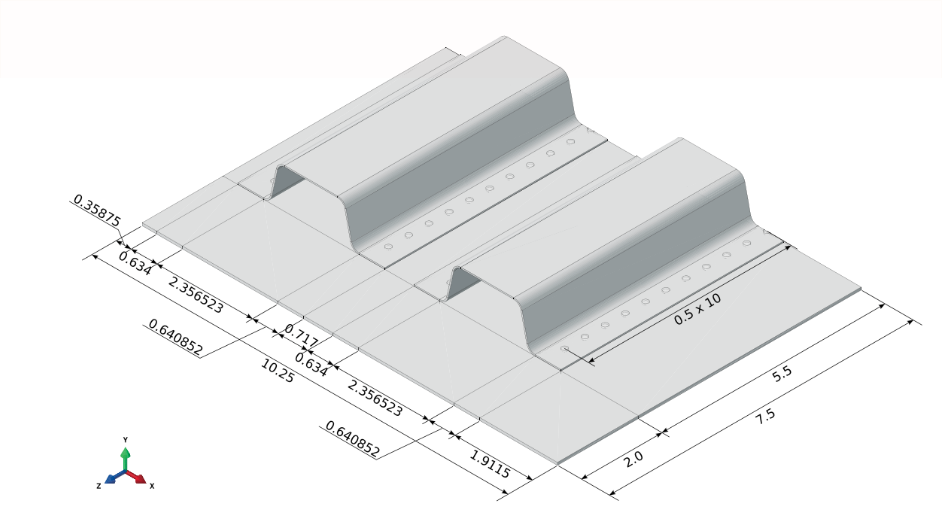
\includegraphics[width=1.1\textwidth]{plews_panel}
\end{figure}

\end{document}
